\newpage
\section{超声波接近传感器总体设计与检测原理}
\subsection{超声波接近传感器总体设计}
在对各部分进行设计之前,首先进行总体设计。本设计的总体设计如图\ref{超声波接近传感器总体设计}所示,包括了超声波接近传感器的硬件设计、软件设计和实验设计。
\begin{figure}[ht]
	\centering
	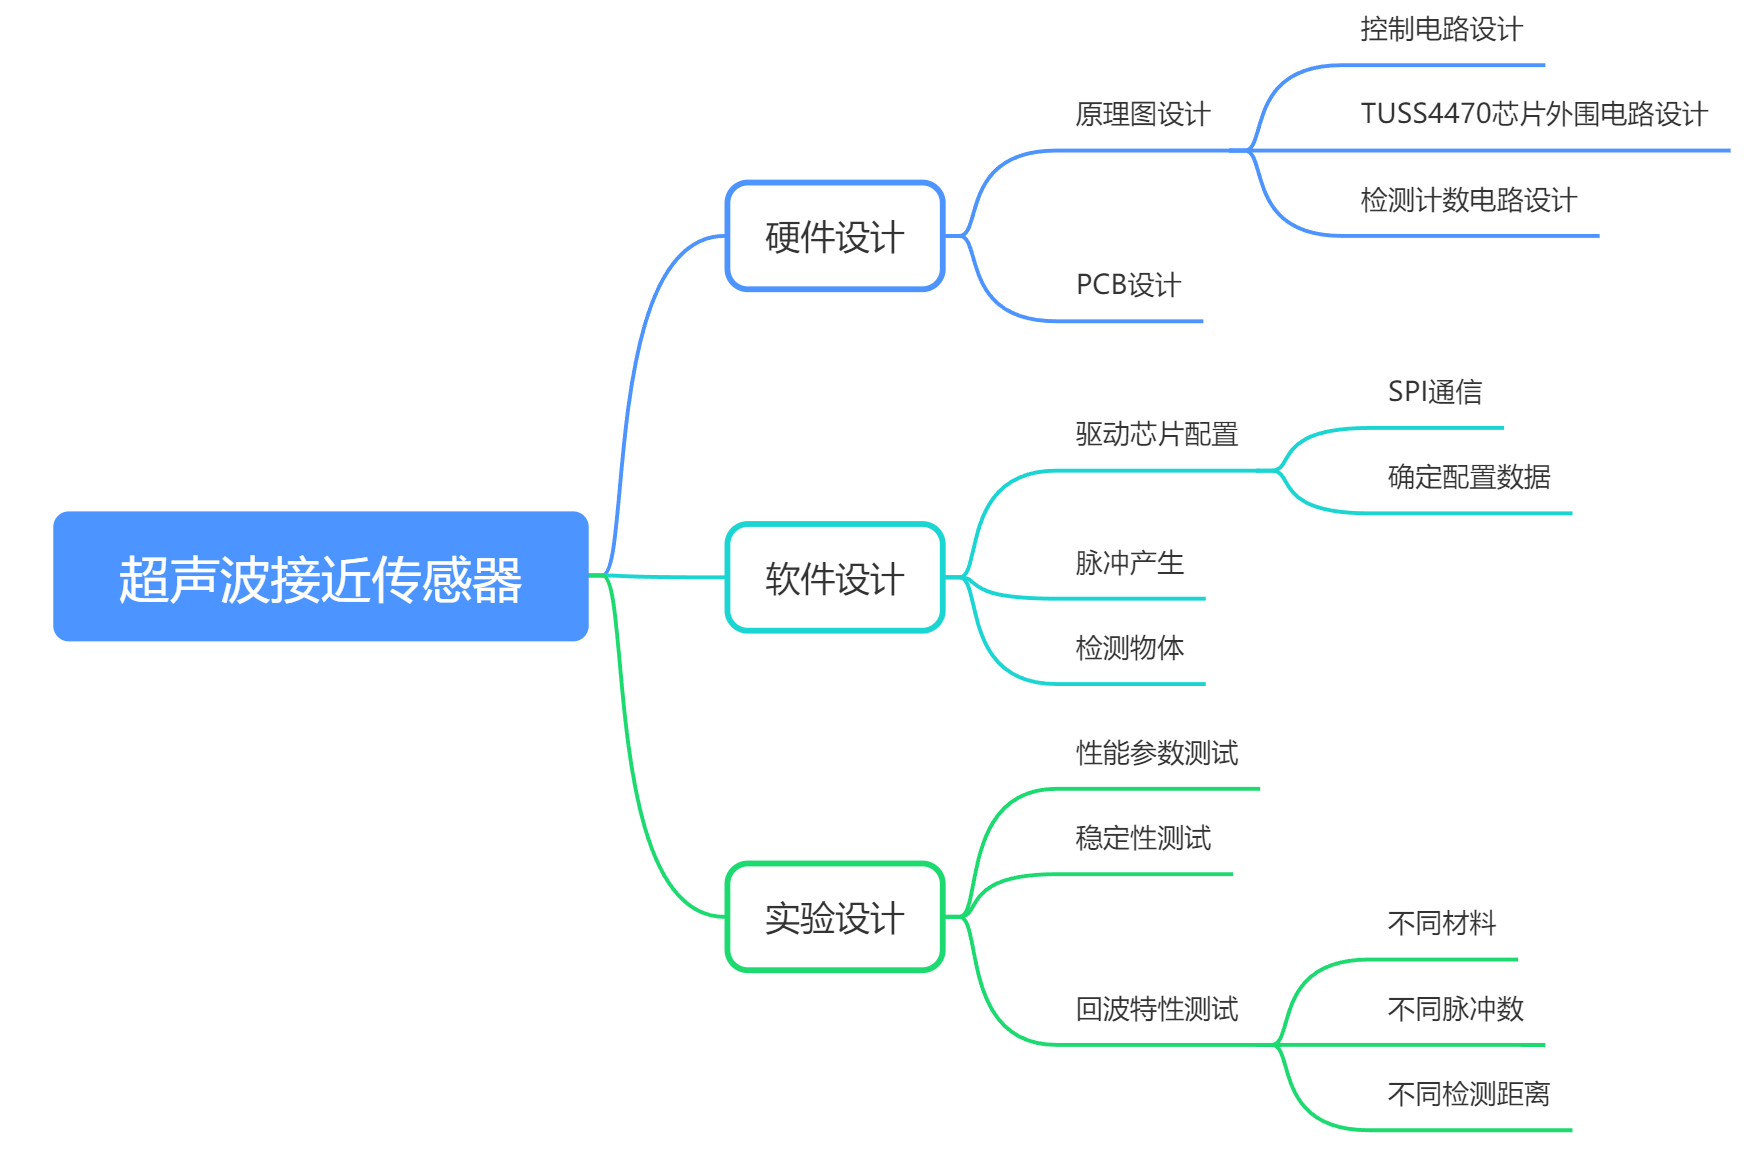
\includegraphics[width=12cm]{figure/overall designment.png}
	\caption{超声波接近传感器总体设计}
	\label{超声波接近传感器总体设计}
\end{figure}

硬件设计部分包括了原理图设计和PCB设计,软件设计包括了驱动芯片配置、脉冲信号产生、物体检测三个部分的程序设计,实验设计部分包括了设计实验进行性能参数测试、稳定性测试和回波特性测试。
\subsubsection{超声波接近传感器硬件设计}
硬件电路原理图的设计主要分为三部分来进行,分别为:超声波接近传感器控制电路设计、TUSS4470芯片外围电路设计、检测计数电路设计。\par
在PCB设计部分,TUSS4470芯片外围电路PCB的设计由为关键,直接关系着传感器准确性,芯片手册根据优先级给出了几大原则,用于减小各类信号相互之间的干扰,包括了电容、二极管等器件摆放位置优先级,分离接地,铺铜规则等。
\subsubsection{超声波接近传感器软件设计}
超声波接近传感器的软件设计根据功能分为了三个部分:芯片配置、脉冲产生、物体检测。\par
通过查找芯片手册,可以得知TUSS4470超声驱动芯片采用四线SPI协议来完成芯片配置,并与MCU进行通信,其采用的模式为CPOL=0、CPHA=1,即上升沿进行数据发送、下降沿进行数据接收,根据查找到的资料,本设计采用线性序列机(linear sequential machine)控制移位寄存器俩实现SPI通信。此外,SPI发送的各寄存器配置数据也需要参照芯片手册,根据应用场景进行确认。\par
在脉冲信号的模式选择上,考虑程序设计难度以及运行速度,本设计选取脉冲模式3来产生脉冲控制信号,即以io2引脚输入的信号作为时钟信号,io1引脚输入的信号为控制信号,两引脚配合工作产生脉冲控制信号。\par
物体检测部分程序主要功能为对回波信号进行处理判断。超声探头发出的脉冲波经物体反射后,重新被传感器所接收,回波信号通过TUSS4470芯片的解调放大处理后,变为简单的回波信号,程序按照检测逻辑对回波信号进行检测判断,从而控制检测状态的转移。
\subsubsection{超声波接近传感器实验设计}
在完成实物的制作与调试后,还需要设计实验来测试传感器的性能以及检测逻辑的可行性。\par
该部分的工作有:测试传感器性能参数、检测策略的可行性以及回波参数特性。性能参数测试包括了检测范围测试和精度测试,检测策略可行性测试关键点在于测试传感器的灵活性,回波特性测试则是为后续的应用提供参考。


\subsection{超声波接近传感器检测原理}
\begin{figure}[!h]
	\centering
	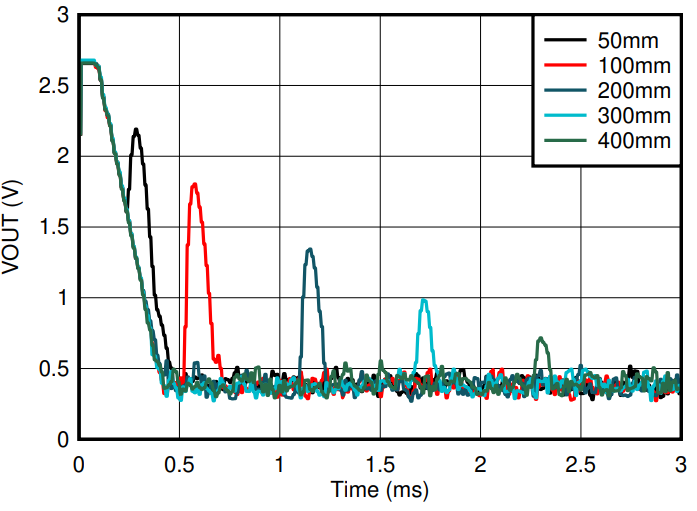
\includegraphics[width=8cm]{figure/VOUT image.png}
	\caption{VOUT输出\upcite{TUSS4470芯片手册}}
	\label{VOUT输出}
\end{figure}\par
通过查阅芯片手册\upcite{TUSS4470芯片手册},我们可以知道,TUSS4470芯片采用的检测原理为飞行时间法,获取飞行时间的方法为固定阈值法。\par
芯片通过滤波解调等处理,可将回波信号处理成一个简单的信号,由VOUT引脚输出,当峰值超过所设定阈值时,即判定为超声换能器接收到回波,该峰值距离起点的时间随检测距离的变化而变化。如图\ref{VOUT输出}所示,当检测物体距离传感器50mm、100mm、200mm、300mm、400mm时,信号的峰值在不断减小,也在不断地向右侧进行移动。但是在到达有效波峰前,仍然存在着一个波峰信号,影响着物体的检测。这是自发自收换能器的弊端,在收到回波时,换能器仍然存在余振,影响回波信号的接收。\par
第二个波峰距离起点的时间$t$由以下公式得出:       
\begin{align}
	t&=t_1+t_2 \\
	t&_2=\frac{D}{b}	
	\label{检测周期公式}
\end{align}  
式中\quad$t$---波峰距离起点时间;\par
\quad$t_1$---脉冲发射时间;\par
\quad$t_2$---飞行时间;\par    
\quad$D$---与检测物体的距离;\par  
\quad$b$---声速\par    
按照任务书的指示,检测范围为100mm-200mm,为简化程序,我们通过设定检测窗口的方式来实现该效果。\par  
当物体与传感器的距离确定时,回波信号波峰对应的$t$也是确定的,该值可以通过实验测得。例如距离为100mm、200mm时,对应t为1.2ms、2.4ms,那么我们可以设定检测窗口为1.2ms-2.4ms,只对这个范围内的波峰进行检测,而屏蔽范围外的信号,从而避免被“盲区”信号所干扰,并且实现检测100mm-200mm范围物体的功能。\par
